\section{Purpose Definition}
% revised
This section introduces the purpose, domain of interest, scenarios and personas, competency questions, and concepts identification for the project.

% Integrate information about student commutes on Trentino transportation with usual places a person goes to and how he felt about the trip/stay at that place 

\subsection{Informal Purpose}
% revised
The objective of this project is to build a knowledge graph that assists students in planning their trips from one location to another using public transportation in an efficient and comfortable manner. This tool aims to facilitate informed decision-making and enhance students' overall university experience. This will be achieved by integrating historical data on student commutes and activities, public transportation information and points of interest.

% revised
\subsection{Domain of Interest}
To focus our attention to what matters most and what are the distinctive features for the entities we will have to be able to handle.s
In this section we outline in which ways we ground our representations to the spatial-temporal domain in the world.

As per the spatial domain of the project, we are focusing our attention on the city of Trento, Italy. In particular, we are mostly interested in the commutes and daily activities of students around the city. For these reasons we identify two main spatial domains of interest: 
   \begin{itemize}
       \item Points of interest in Trento that students are interested in, such as bars, libraries, restaurants, ...
        \item Public transportation bus stops locations
   \end{itemize}
   
While the main focus for the temporal domain is driven by the need to model the bus routes. For this reason, the distinction we have to make is into two classes:
   \begin{itemize}
        \item weekdays
        \item festive days
   \end{itemize}
% A note should be made about the daytime and nighttime routes, but those can be handled by defining the timetable for each bus during an entire day, while it would explode in combinations if had to to do this for each day.

One interesting domain that we are interested in exploring is the state of crowdedness of places or routes and the emotional state of students. While this information can be grounded in the world by the location and the time at which it occurs, we also need to define their respective domains:
\begin{itemize}
    \item The crowdedness state can take one of these four values: empty, low, high, full.
    \item The emotional state following the iLog data format is mapped to a scale from 0 to 5.
\end{itemize}
    
\subsection{Personas \& Scenarios definition}
In this section, we introduce the personas and scenarios to ground the purpose on possible use-case of actual users of our knowledge graph.

% revised
\subsubsection{Personas}
To formalize the purpose of the project, we provide personas that covers various lifestyles among student which are useful to define diverse interactions with the knowledge graph.

\begin{description}
    \item[Person 1] Alessia, a new international student, has recently started studying at the university.
    \item[Person 2] Paolo, a second-year master's student. 
    \item[Person 3] Houda, an Erasmus student who wants to save up money
    \item[Person 4] Lucia, a student habit of dining in restaurant quite frequently
    \item[Person 5] Emanuele, a student who lives in San Bartolomeo student residence
\end{description}

% revised
\subsubsection{Scenarios}
For the persons we defined, we described some scenarios students could encounter during their university lifestyle in which our Knowledge Graph can assist for making decisions on planning.

\begin{enumerate}
    \item \textbf{Social Interaction} - Alessia has recently moved to Italy and is excited to spend time with her new friends, exploring the city center of Trento, as she is eager to get to know the city.
    \item \textbf{University Facilities} - Paolo is a second-year master's student at the University of Trento, currently working on his thesis. He wants to study in a quiet, uncrowded place, so he needs to choose one of the university's facilities.
    \item \textbf{Daily life} - As an exchange student, Houda has started living in the city center and is planning to go grocery shopping. Since the atmosphere in supermarkets varies, he wants to choose the one that best suits his preferences.
    \item \textbf{Dinner Place} - Regarding her dining habits, Lucia is looking for decent places to have dinner with her flatmate. While exploring restaurants she had both good and bad experiences in plates, so she doesn't want to choose a bad one.
    \item \textbf{Personal Activity - } Emanuele is a professional athlete looking to have permanent training at the nearest sports facility to his student residence. A regular commute to the facility is an important part of his daily routine, so he needs to choose the one that will save him time.
\end{enumerate}

\subsection{Competency Questions}
Following the paper on \href{https://arxiv.org/pdf/2409.05883}{Big-Thick Data generation via reference and personal context unification}, what we want to be able to answer are about personal-reference (PR) and reference-personal (RP) context questions.
The following is a list of relevant questions for the scenarios and personas we defined which align with the purpose of our Knowledge Graph:

%  grammar checked
\begin{enumerate}
    \item \textbf{P1-S1 PR}. Is public transport available to reach the destination?
    \item \textbf{P1-S1}. Is the bus to the destination full, or does it have enough space for the group members?
    \item \textbf{P1-S1}. How crowded are the social interaction locations in the city?
    \item \textbf{P2-S2}. Which university facility best fits the student's needs or has the least impact on their mood?
    \item \textbf{P2-S2}. How crowded is BUC?
    \item \textbf{P3-S3}. Which supermarket best meets the student's needs?
    \item \textbf{P3-S3}. What was the student's mood when they were at the Coop supermarket?
    \item \textbf{P3-S3}. What is the best route to the Coop supermarket?
    \item \textbf{P3-S3}. How did I feel about the trip to the Coop supermarket when it was crowded?
    \item \textbf{P4-S4}. Which restaurant served a meal that met the student's expectations?
    \item \textbf{P5-S5}. Which sports facility is closest to the student's residence?
    \item \textbf{P5-S5}. What is the best bus route to the sports facility?
    \item \textbf{P5-S5}. What is the closest bus stop to reach the facility?


%\newline
%(PR - person-reference, RP - reference-person)
\end{enumerate}

\subsection{Concepts Identification}
In this section, we try to come up with a mostly complete list and description of what type of concepts we are interested in modeling and which properties are fundamental for the Knowledge Graph.
In the next section, we will use this information to guide the modeling of the ER diagram.

\begin{table}[ht]
    \centering
    \begin{tabular}{|c|c|c|c|c|l|} \hline 
         Scenarios&  Personas&  CQs&  Entities& Properties &Focus\\ \hline 
         1-5&  1-5&  1-11&  Student&  student\_id, name, current\_position&Contextual\\ \hline 
         %1, &  1, 2&  1, 2, 8, 9&  Bus&  vehicle\_id, number,&Common\\ \hline 
1, 5&  1, 5&  1, 13&  Bus Stop&  name, direction, time\_table, location&Contextual\\ \hline 
         3, 5&  2, 5&  2, 8, 12&  Bus route&  number, festive, start\_time&Contextual\\ \hline
 4& 4& 10& Restaurant& civic\_number, name, location&Common\\\hline
 2& 2& 3-5& Univercity Facility& civic\_number, name, location&Common\\\hline
 5& 5& 11& Sport Facility& civic\_number, name, location&Common\\\hline
 1& 1& 3& Bar& civic\_number, name, location&Common\\\hline
 5& 5& 11& Residence& intercom\_name, civic\_number, location&Contextual\\ \hline 
 3& 3& 6-9& Supermarket& civic\_number, name, location&Common\\\hline
 2-4& 2-4& 4,7,9-10& Emotional state& time, duration, location, user, mood&Core\\\hline
 1-3& 1-3& 2-5,9& Crowdedness state& time, duration, location, density&Core\\\hline
    \end{tabular}
    \caption{Concepts Identification table}
    \label{tab:entity_table}
\end{table}

Table \ref{tab:entity_table} reports the identified concepts and relates each to the specific competency question in which their use is required to correctly answer them.
The most important concepts we identified for this part are the \textbf{Emotional State} and the \textbf{Crowdedness State} which will be used by our Knowledge Graph to address the majority of the reference-to-personal and personal-to-reference queries we aim to tackle.

\subsection{ER modeling}

Having defined the specific concept instances relevant to our identified competency questions, we now aim to formalize the newly acquired insights. 
To do so, we use the Entity-Relationship (ER) modeling to identify and define the entity types that we will need to manage and use.
The resulting model is depicted in the image. \ref{fig:ER-model}.

\begin{figure}
    \centering
    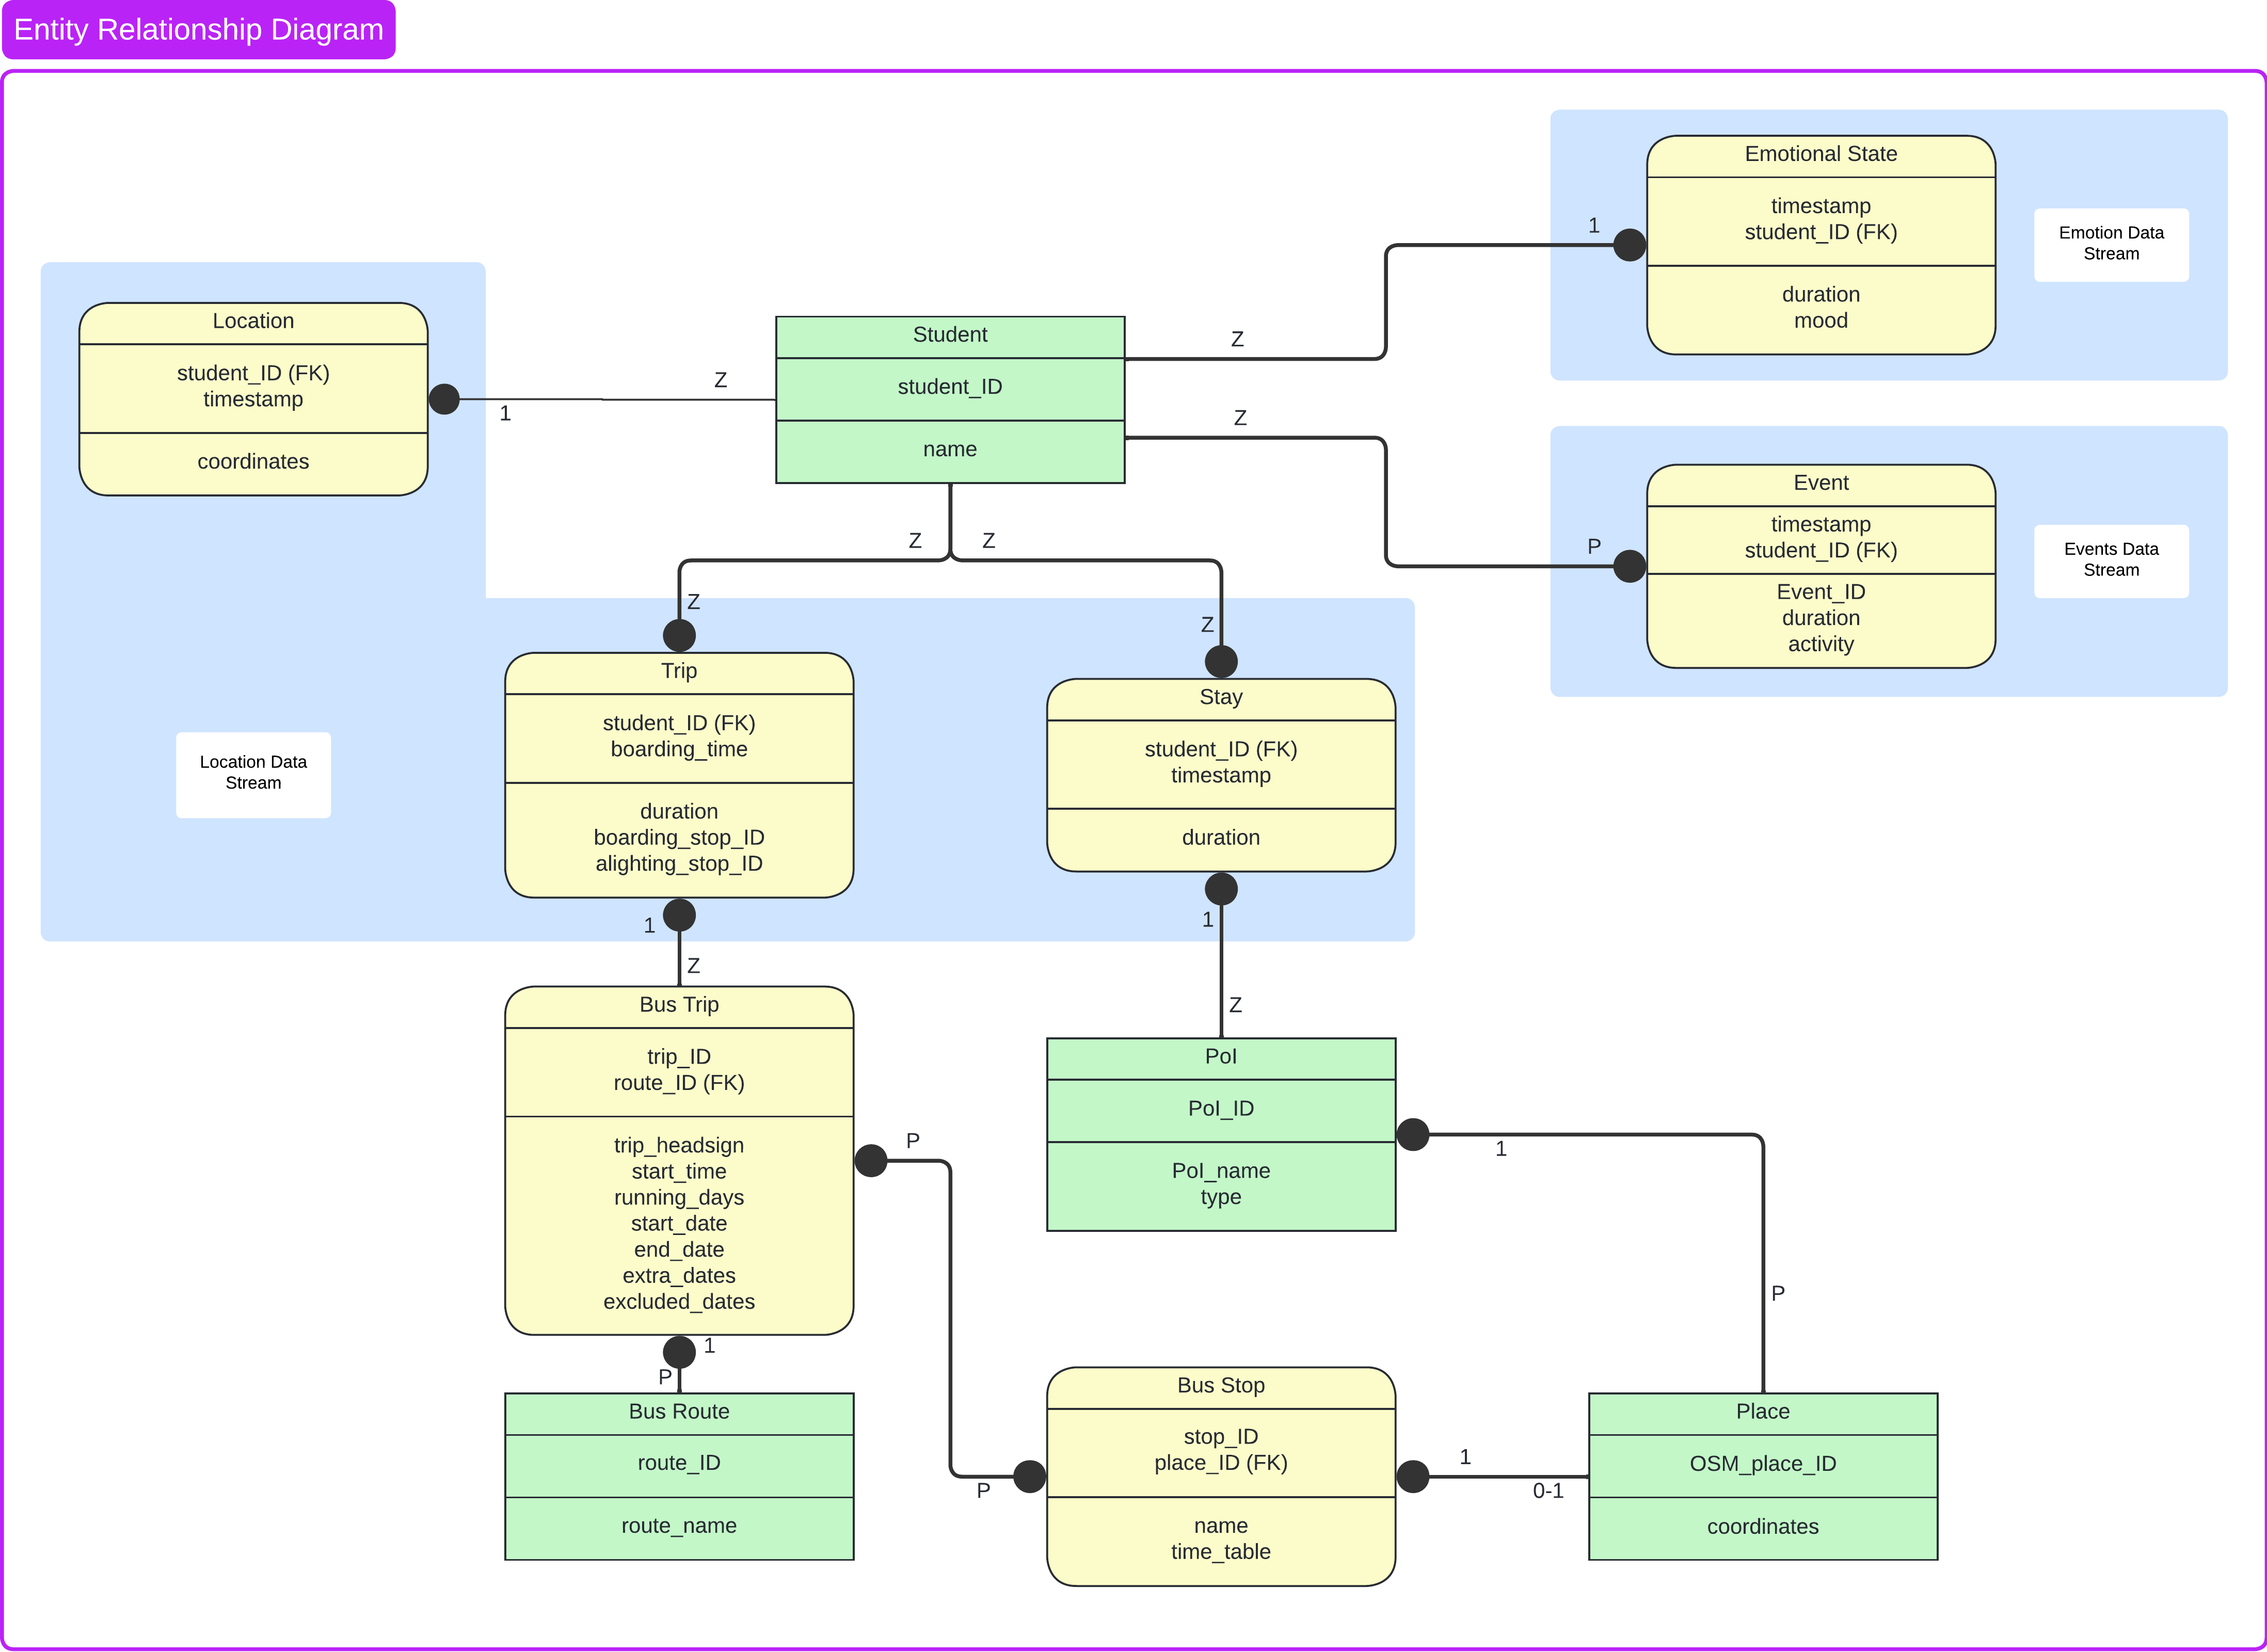
\includegraphics[width=0.8\linewidth]{images/ER diagram.png}
    \caption{ER model}
    \label{fig:ER-model}
\end{figure}

% rivesed
During the modeling process, we encountered several design choices.. 

One comes from the realization that, in all the questions we defined, we are only interested only in a subset of places that satisfy specific requirements, such as being suitable for hanging out with friends, having dinner, or working out. 
Therefore, it was unnecessary to model each place (e.g., restaurant, bar, sports facility) as a separate entity in the ER model.
Instead, we collapsed them under a single \textbf{PoI} (Point of Interest) entity, differentiated by a \textit{type} property.

Another important design choice is the need to separate the concepts of \textbf{Emotional state} and \textbf{Crowdedness state} used to describe a location from those used to describe a bus route.
This is dictated by the No-Null and No-Repetition rules, which prevent us from collapsing these states into a single entity.


